
\documentclass[11pt]{article}
\usepackage[margin=0.8in]{geometry}
\usepackage{amsmath,amssymb,booktabs,array,longtable}
\usepackage{hyperref}
\usepackage{graphicx}
\usepackage{float}
\usepackage{enumitem}
\setlist{nosep}

\begin{document}

\begin{center}
{\Large\textbf{Shiv Nadar University Chennai}}\\
\textbf{CS3807 -- Deep Learning Laboratory}\\
\textbf{Experiment 2}\\
{\large\textbf{Implementation of a Multi-Layer Perceptron (MLP) for Multi-Class Image Classification}}
\end{center}

\renewcommand{\arraystretch}{1.25}

\begin{tabular}{|p{3.8cm}|p{8cm}|p{2cm}|}
\hline
Degree \& Branch & B.Tech Artificial Intelligence \& Data Science & Semester V\\ \hline
Subject Code \& Name & CS3807 -- Deep Learning Laboratory & AY: 2026--27\\ \hline
\end{tabular}

\section*{1. Objective}
Implement an MLP using TensorFlow/Keras on the Fashion-MNIST dataset. Learn image preprocessing, flattening, model construction, training, evaluation, and automated hyperparameter optimization.

\section*{2. Background Theory}
An MLP consists of an input layer, hidden layers and an output layer.

\[
z^{(l)}=W^{(l)}a^{(l-1)}+b^{(l)},\qquad
a^{(l)}=f(z^{(l)})
\]

Output layer:
\[
\hat y=\mathrm{Softmax}(z)
\]

Loss:
\[
L=-\sum_i y_i\log(\hat y_i)
\]

Recommended architecture:

\begin{center}
784 $\rightarrow$ Dense(128, ReLU) $\rightarrow$ Dense(64, ReLU) $\rightarrow$ Dense(10, Softmax)
\end{center}

\section*{3. Dataset}
Dataset: Fashion-MNIST

Training Images: 60,000 \\
Testing Images: 10,000 \\
Classes: 10 \\
Image Size: $28\times28$

\section*{4. Experimental Procedure}

\textbf{Task 1: Dataset Exploration}
\begin{itemize}
\item Load Fashion-MNIST.
\item Print dataset dimensions.
\item Display ten sample images.
\item Plot class distribution.
\end{itemize}

\textbf{Expected Output:}
Dataset summary and sample images.

\bigskip

\textbf{Task 2: Data Preprocessing}

\begin{itemize}
\item Flatten images.
\item Normalize pixel values.
\item Print tensor shapes before and after preprocessing.
\end{itemize}

\bigskip

\textbf{Task 3: Model Construction}

Construct an MLP with

\begin{itemize}
\item Input layer (784)
\item Dense(128, ReLU)
\item Dense(64, ReLU)
\item Dense(10, Softmax)
\end{itemize}

Display \texttt{model.summary()}.

\bigskip

\textbf{Task 4: Model Training}

Compile using

\begin{itemize}
\item Optimizer: Adam
\item Loss: Categorical Cross Entropy
\item Metric: Accuracy
\end{itemize}

Train for 20 epochs with batch size 32.

\bigskip

\textbf{Task 5: Model Evaluation}

Compute

\begin{itemize}
\item Accuracy
\item Precision
\item Recall
\item F1-score
\item Confusion Matrix
\item Classification Report
\end{itemize}

\section*{5. Source Code}

The complete source code is attached separately in the GitHub repository and submitted along with this report.

\textbf{GitHub Repository:}

\url{https://github.com/Sadhana2006-art/Deep-Learning-Lab}

\section*{6. Hyperparameter Optimization}

Instead of manually selecting hyperparameters, students shall perform automated hyperparameter optimization using either \textbf{GridSearchCV} or \textbf{RandomizedSearchCV} (recommended) together with the SciKeras wrapper.

Optimize the following search space.

\begin{center}
\begin{tabular}{|p{5cm}|p{7cm}|}
\hline
Hyperparameter & Candidate Values\\
\hline
Hidden Layers & 1, 2, 3\\
Hidden Neurons & 32, 64, 128, 256\\
Learning Rate & 0.1, 0.01, 0.001\\
Batch Size & 16, 32, 64, 128\\
Epochs & 10, 20, 30\\
Optimizer & SGD, Adam, RMSProp\\
Activation Function & ReLU, Tanh, Sigmoid\\
Dropout Rate (Optional) & 0.0, 0.2, 0.5\\
\hline
\end{tabular}
\end{center}

\subsection*{Tasks}

\begin{enumerate}
\item Build a baseline MLP model.
\item Define the hyperparameter search space.
\item Perform Grid Search or Randomized Search using 5-fold cross-validation.
\item Record the best hyperparameter combination.
\item Retrain the model using the optimized hyperparameters.
\item Evaluate the optimized model on the testing dataset.
\item Compare the optimized model with the baseline model.
\end{enumerate}

\section*{7. Results}

\textbf{Best Hyperparameters}

\begin{tabular}{|p{6cm}|p{6cm}|}
\hline
Hidden Layers & 1 \\
\hline
Hidden Neurons & 128 \\
\hline
Learning Rate & 0.1 \\
\hline
Batch Size & 32 \\
\hline
Optimizer & sgd \\
\hline
Activation Function & Tanh \\
\hline
Epochs & 30 \\
\hline
Dropout & 0.0 \\
\hline
Cross-validation Accuracy & 0.8863 (88.63\%)\\
\hline
Testing Accuracy & 0.8862 (88.62\%)\\
\hline
\end{tabular}

\vspace{3mm}

\textbf{Performance Comparison}

\begin{tabular}{|p{4cm}|c|c|}
\hline
Metric & Baseline & Optimized\\
\hline
Accuracy& 0.888100 & 0.886200 \\
Precision& 0.888441 & 0.888336 \\
Recall& 0.888100 & 0.886200 \\
F1-score& 0.888136 & 0.885920 \\
Training Time& 151.424753 & 162.067963 \\
\hline
\end{tabular}

\section*{8. Plots with Inference}

\subsection{Sample Images}

\begin{figure}[H]
\centering
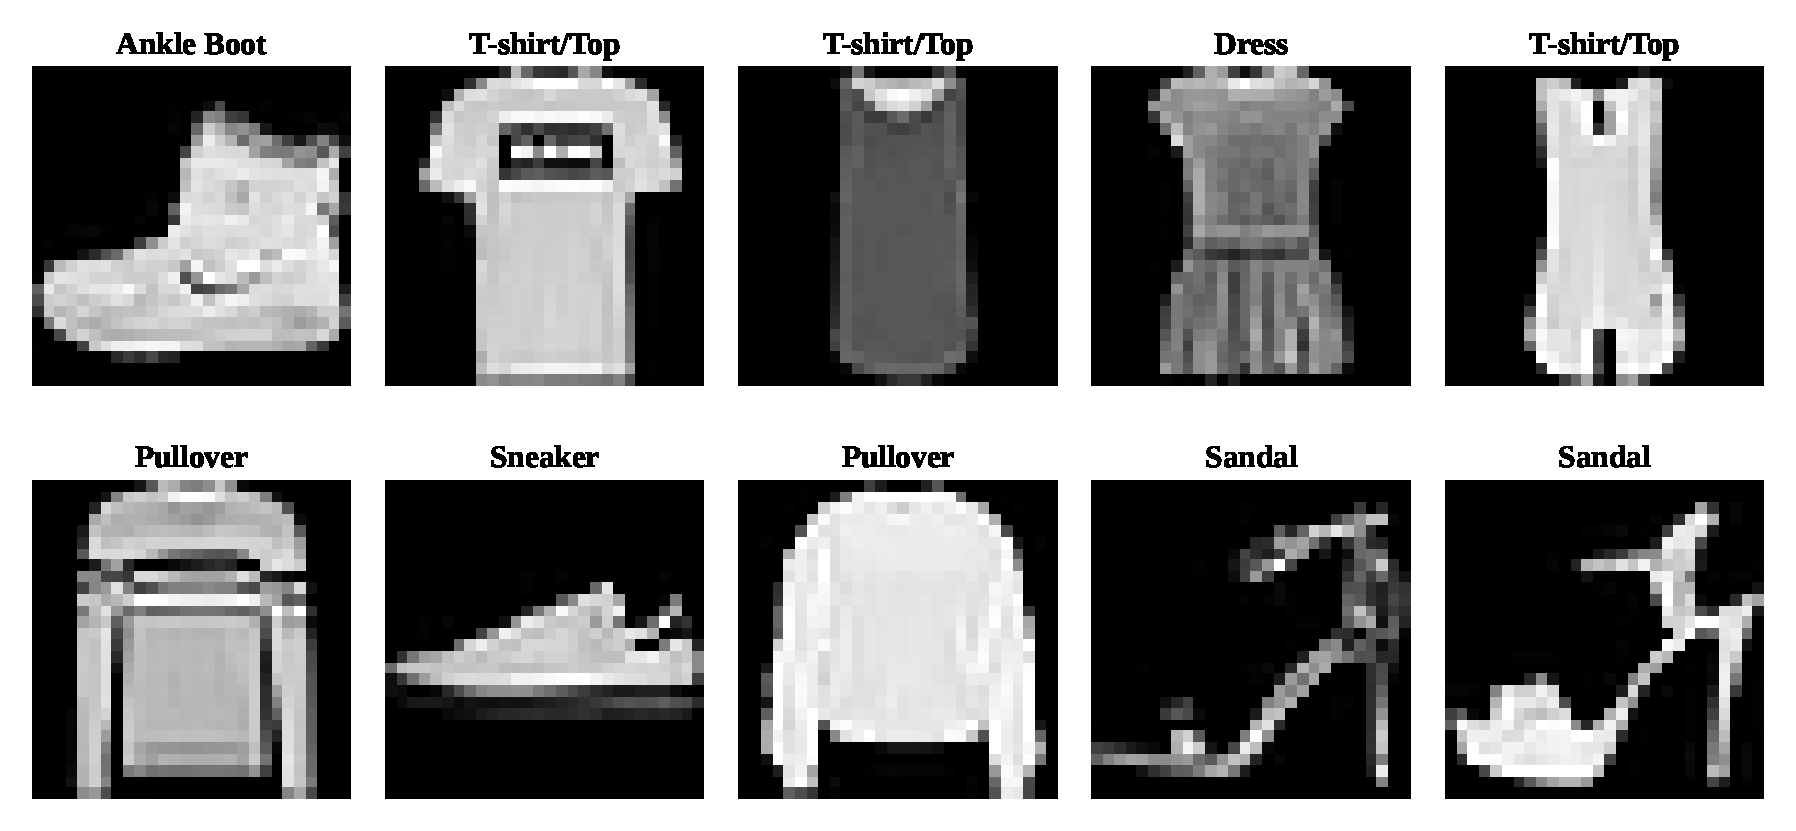
\includegraphics[width=\textwidth]{Sample_Images.eps}
\caption{Sample Images from the Dataset}
\end{figure}

\textbf{Interpretation:}

Figure displays ten sample images from the Fashion-MNIST dataset, which are different types of clothing such as t-shirts, dresses, pullovers, sandals, sneakers and ankle boots. The images are in grey-scale with a resolution of 28 × 28 pixels.This confirms that the dataset is loaded properly.

\subsection{Class Distribution}

\begin{figure}[H]
\centering
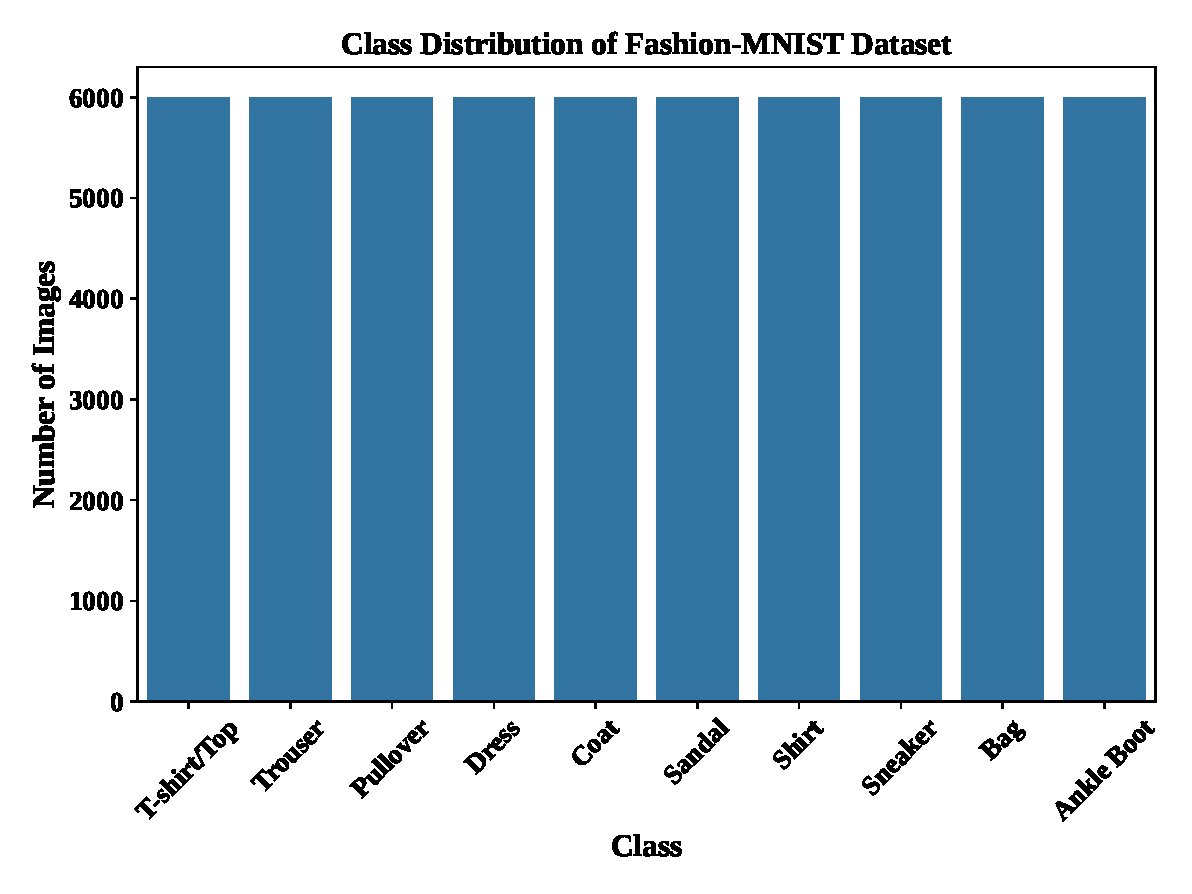
\includegraphics[width=\textwidth]{Class_Distribution.eps}
\caption{Distribution of Classes in the Dataset}
\end{figure}

\textbf{Interpretation:}

The dataset is evenly distributed which is a balanced dataset among the ten classes, with each class having around 6,000 images. This uniform distribution helps ensure fair model training and improves the robustness of the classification results.

\subsection{Training Accuracy vs Epoch}

\begin{figure}[H]
\centering
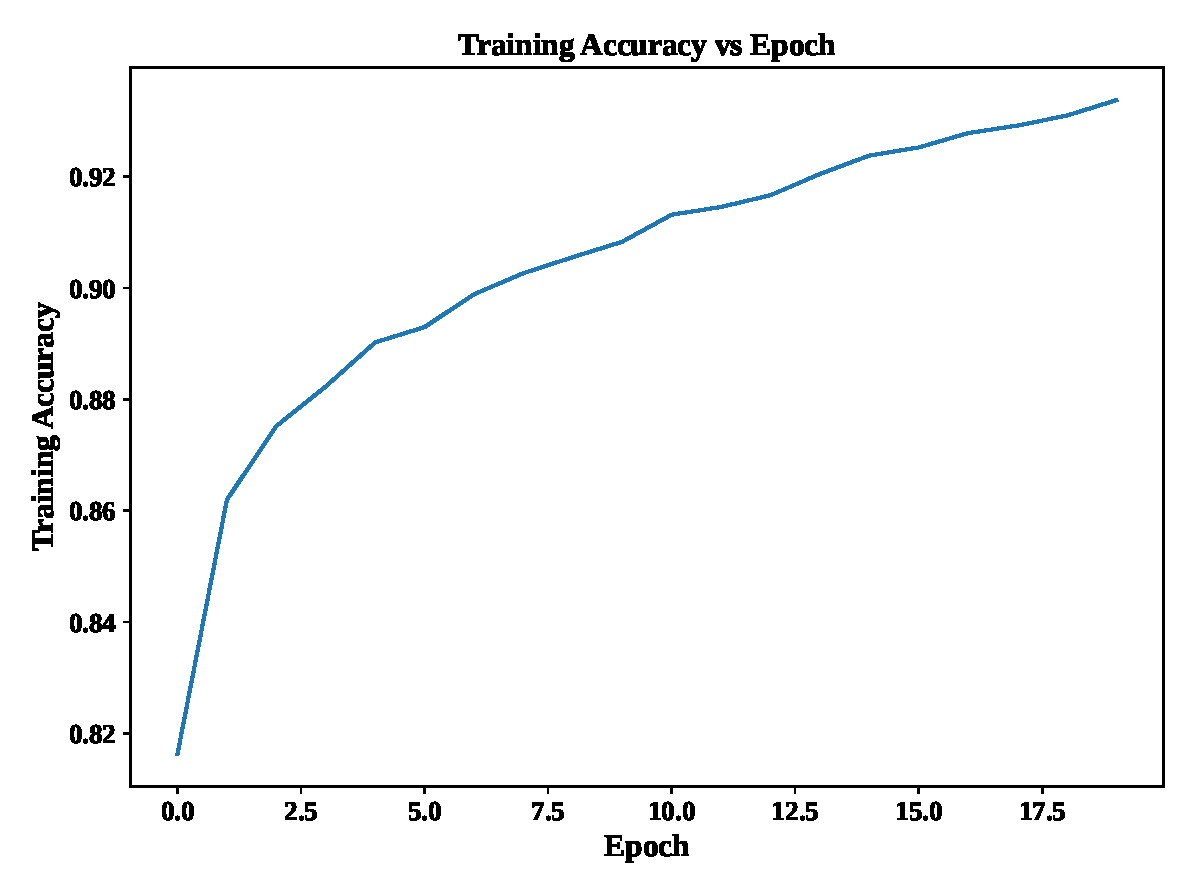
\includegraphics[width=\textwidth]{Training_Accuracy_vs_Epoch.eps}
\caption{Training Accuracy versus Epoch}
\end{figure}

\textbf{Interpretation:}

The training accuracy shows a gradual growth through the 20 epochs indicating that the MLP model is learning well. The curve gradually stabilises in the later epochs, suggesting that the model is converging to an optimal solution without significant fluctuations.

\subsection{Validation Accuracy vs Epoch}

\begin{figure}[H]
\centering
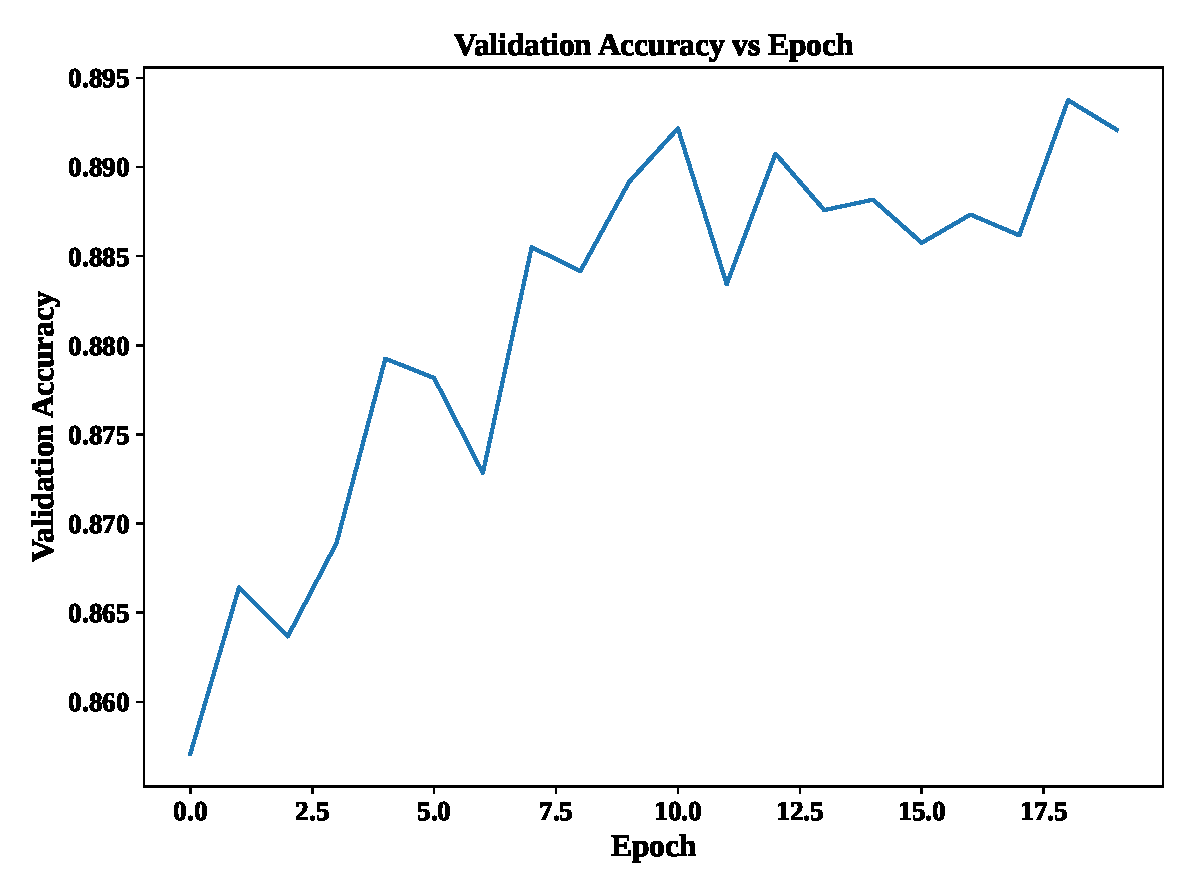
\includegraphics[width=\textwidth]{Validation_Accuracy_vs_Epoch.eps}
\caption{Validation Accuracy vs Epoch}
\end{figure}

\textbf{Interpretation:}

The validation accuracy increases gradually during training and converges to an approximately 89\% accuracy, which shows that the model learns well and generalises well. 

\subsection{Training Loss vs Epoch}

\begin{figure}[H]
\centering
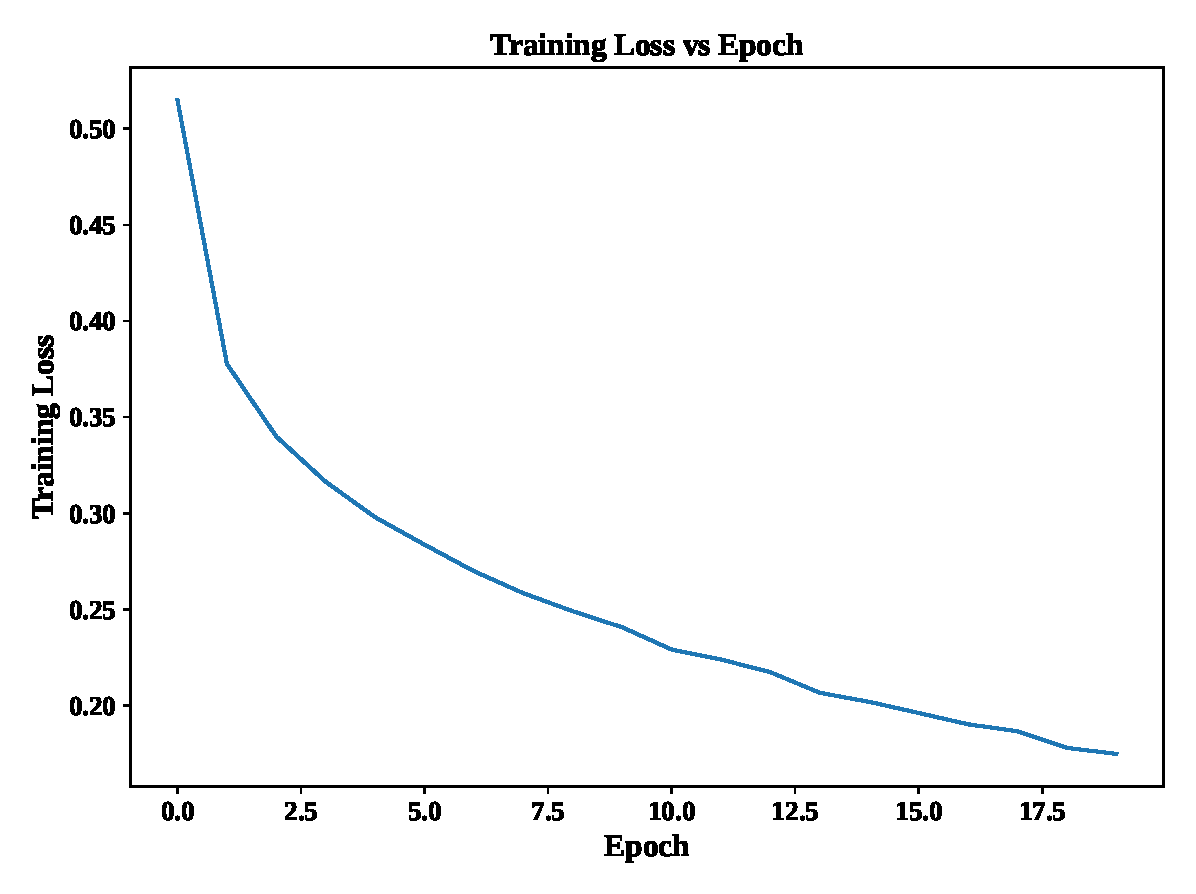
\includegraphics[width=\textwidth]{Training_Loss_vs_Epoch.eps}
\caption{Training Loss versus Epoch}
\end{figure}

\textbf{Interpretation:}

The training loss decreases consistently during the training, which means that the MLP is improving its predictions by minimising the error. The absence of sudden spikes indicates that the optimisation is stable and the learning algorithm converges successfully.

\subsection{Validation Loss vs Epoch}

\begin{figure}[H]
\centering
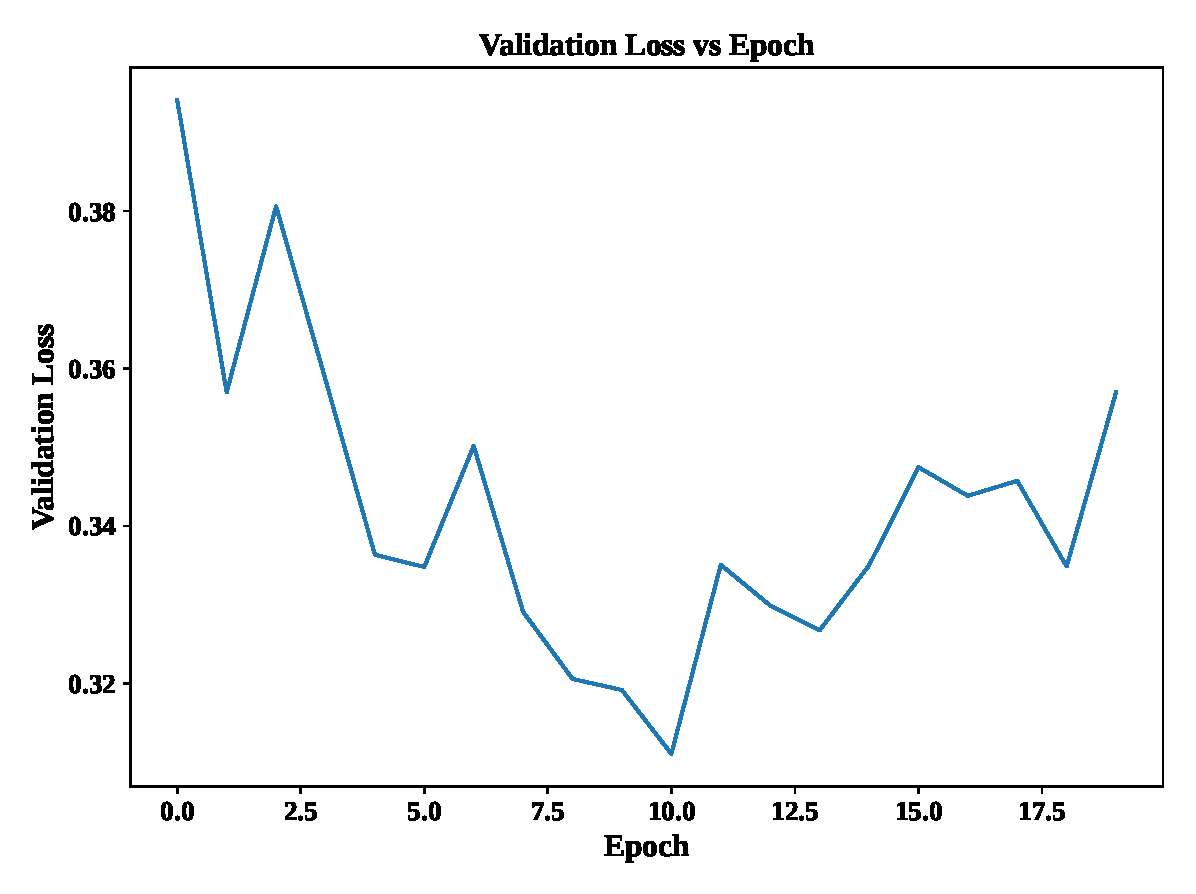
\includegraphics[width=\textwidth]{Validation_Loss_vs_Epoch.eps}
\caption{Validation Loss versus Epoch}
\end{figure}

\textbf{Interpretation:}

In the first few training epochs, the validation loss decreases and reaches its minimum around the middle of training, which indicates an improvement in performance on unseen validation data. The minor fluctuations in the last epochs indicate marginal changes in generalisation and the model is stable without significant overfitting.

\subsection{Confusion Matrix}

\begin{figure}[H]
\centering

\includegraphics[width=0.75\textwidth]{Confusion_Matrix.eps}
\caption{Confusion Matrix}
\end{figure}

\textbf{Interpretation:}

It is seen from the confusion matrix that the predictions tend to lie on the diagonal, which means that the MLP correctly predicts most of the images. Some mistakes in classification happen between those classes that look alike, namely T-shirt/Top – Shirt, Pullover – Coat, and Sneaker – Ankle Boot.

\subsection{Hyperparameter Search Results}

\begin{figure}[H]
\centering
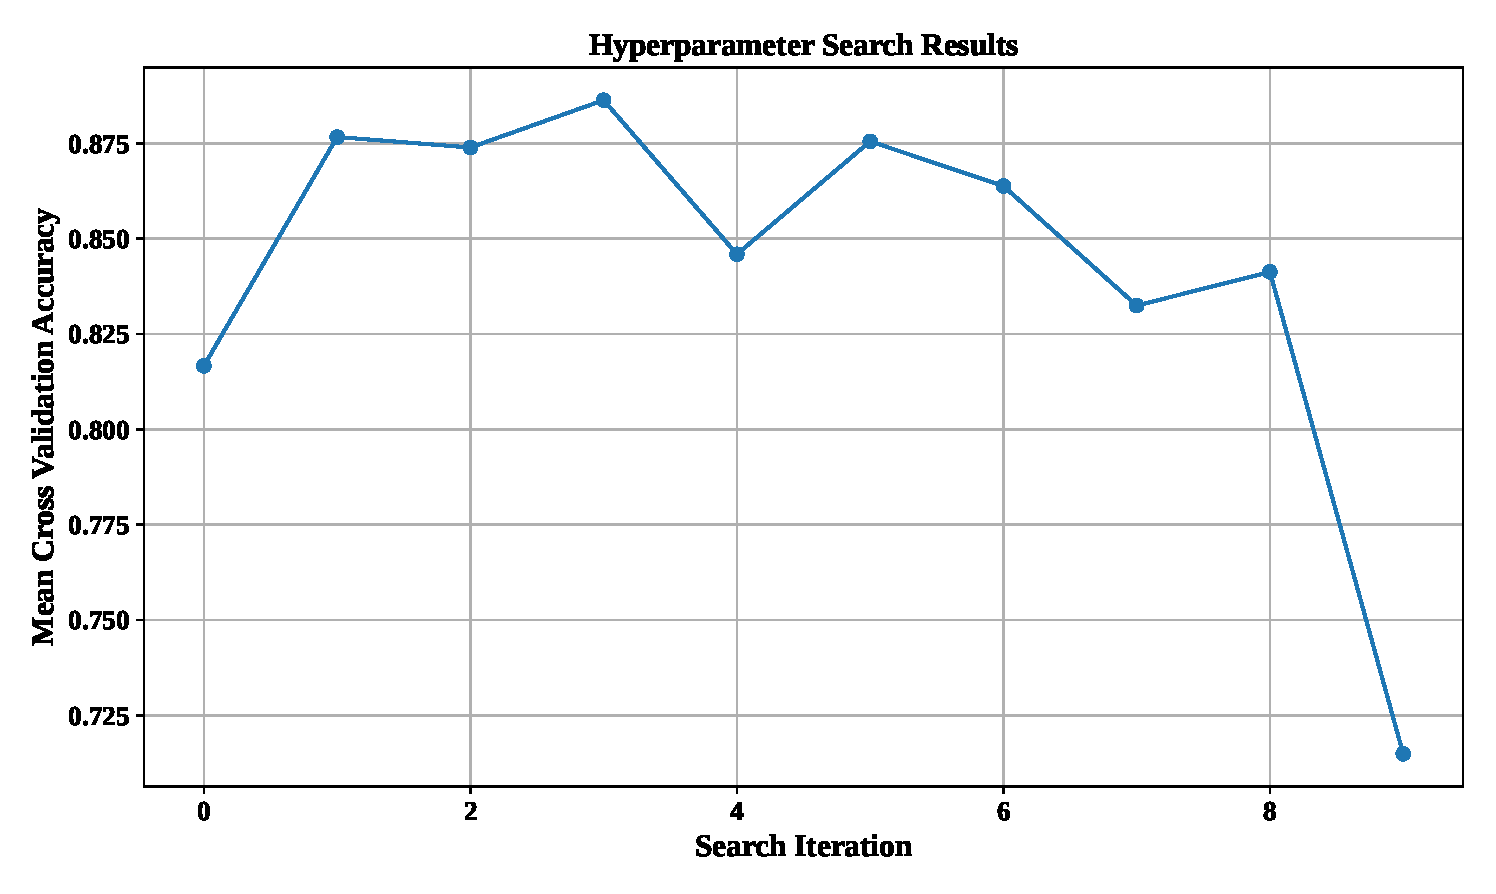
\includegraphics[width=0.9\textwidth]{Hyperparameter_Search_Results.eps}
\caption{Hyperparameter Search Results}
\end{figure}

\textbf{Interpretation:}

Multiple combinations of hyperparameters were tried during the Randomized Search and this was done using 5-fold cross validation. Out of all the different combinations tried, Iteration 3 produced the best mean cross validation accuracy of 88.63\% and this combination was used to train the optimized MLP.

\subsection{Best Model Accuracy Comparison}

\begin{figure}[H]
\centering
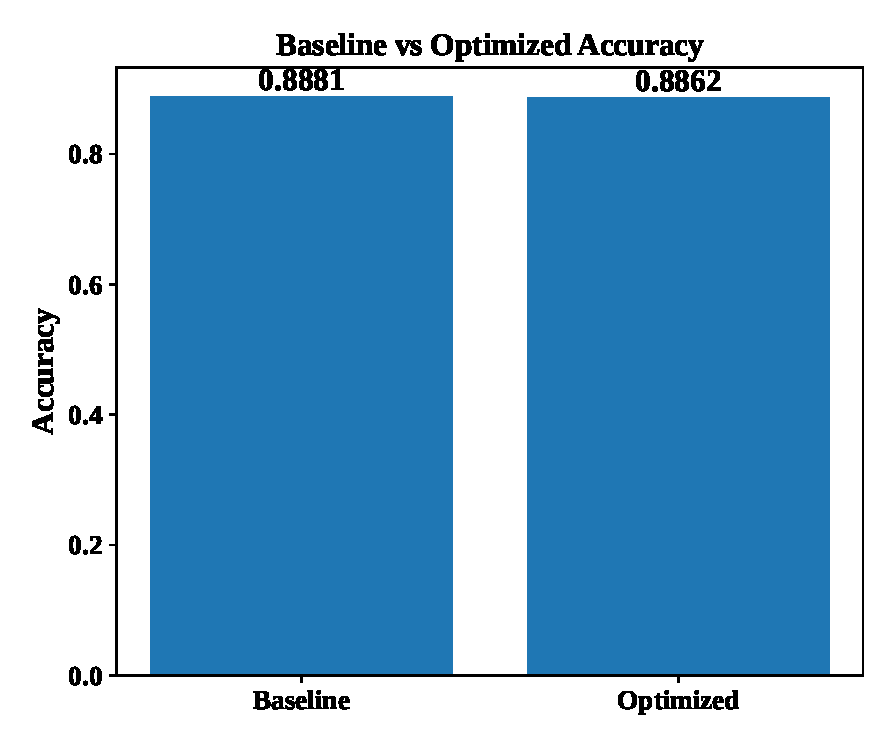
\includegraphics[width=0.9\textwidth]{Accuracy_Comparison.eps}
\caption{Best Model Accuracy Comparison}
\end{figure}

\textbf{Interpretation:}

The accuracy for the optimized MLP model on the test set was 88.62\% compared to 88.81\% of the baseline model, meaning that there was no significant change in performance but only in the model's architecture through hyperparameter optimization.

\section*{9. Discussion}

\begin{enumerate}[leftmargin=*]
\item \textbf{Which optimization method was used?}

RandomizedSearchCV with 5-fold cross-validation along with SciKeras KerasClassifier wrapper was utilized. In this method, a random combination of hyperparameters is picked and the model that gives maximum accuracy in terms of cross-validation is chosen.

\item \textbf{Which hyperparameters were selected?}

In Randomized Search, one hidden layer, 128 neurons, Tanh activation, SGD optimization with learning rate of 0.1, batch size of 32, number of epochs of 30, and dropout of 0.0 were chosen which resulted in a cross-validation accuracy of 88.63\%.

\item \textbf{Did optimization improve performance?}

In comparison to the baseline model whose accuracy is 88.81\% in testing, the optimized model's accuracy is only 88.62\%. Thus, optimization does not result in a better final testing accuracy but a comparable model is obtained with a hyperparameter setting that is selected automatically.

\item \textbf{Which hyperparameter had the greatest impact?}

The optimizer, learning rate, and activation function made the most significant effect on the results of the neural network. The combination of various values of these hyperparameters led to differences in the results of cross-validation.

\item \textbf{Compare Grid Search and Randomized Search.}

Grid Search tries all possible values of hyperparameters, which makes it costly computationally but exhaustive. On the other hand, Randomized Search considers only randomly selected values of hyperparameters, which makes it less costly and faster but still generates near-optimal results.

\item \textbf{Recommend the best MLP configuration.}

According to the Randomized Search, the suggested MLP architecture is as follows:

Input Layer: 784 nodes,
Hidden Layers: 1,
Hidden Nodes: 128,
Activation Function: Tanh,
Optimizer: SGD,
Learning rate: 0.1,
Batch size: 32,
Epochs: 30,
Dropout: 0.0,
Output Layer: 10 nodes with Softmax activation

It provided the highest cross-validation accuracy (88.63\%) while keeping the testing accuracy (88.62\%) equal to that of the baseline architecture.

\end{enumerate}

\section*{10. Additional tasks}

\subsection{Perceptron learning algorithm for XOR Gate}

\begin{figure}[H]
\centering
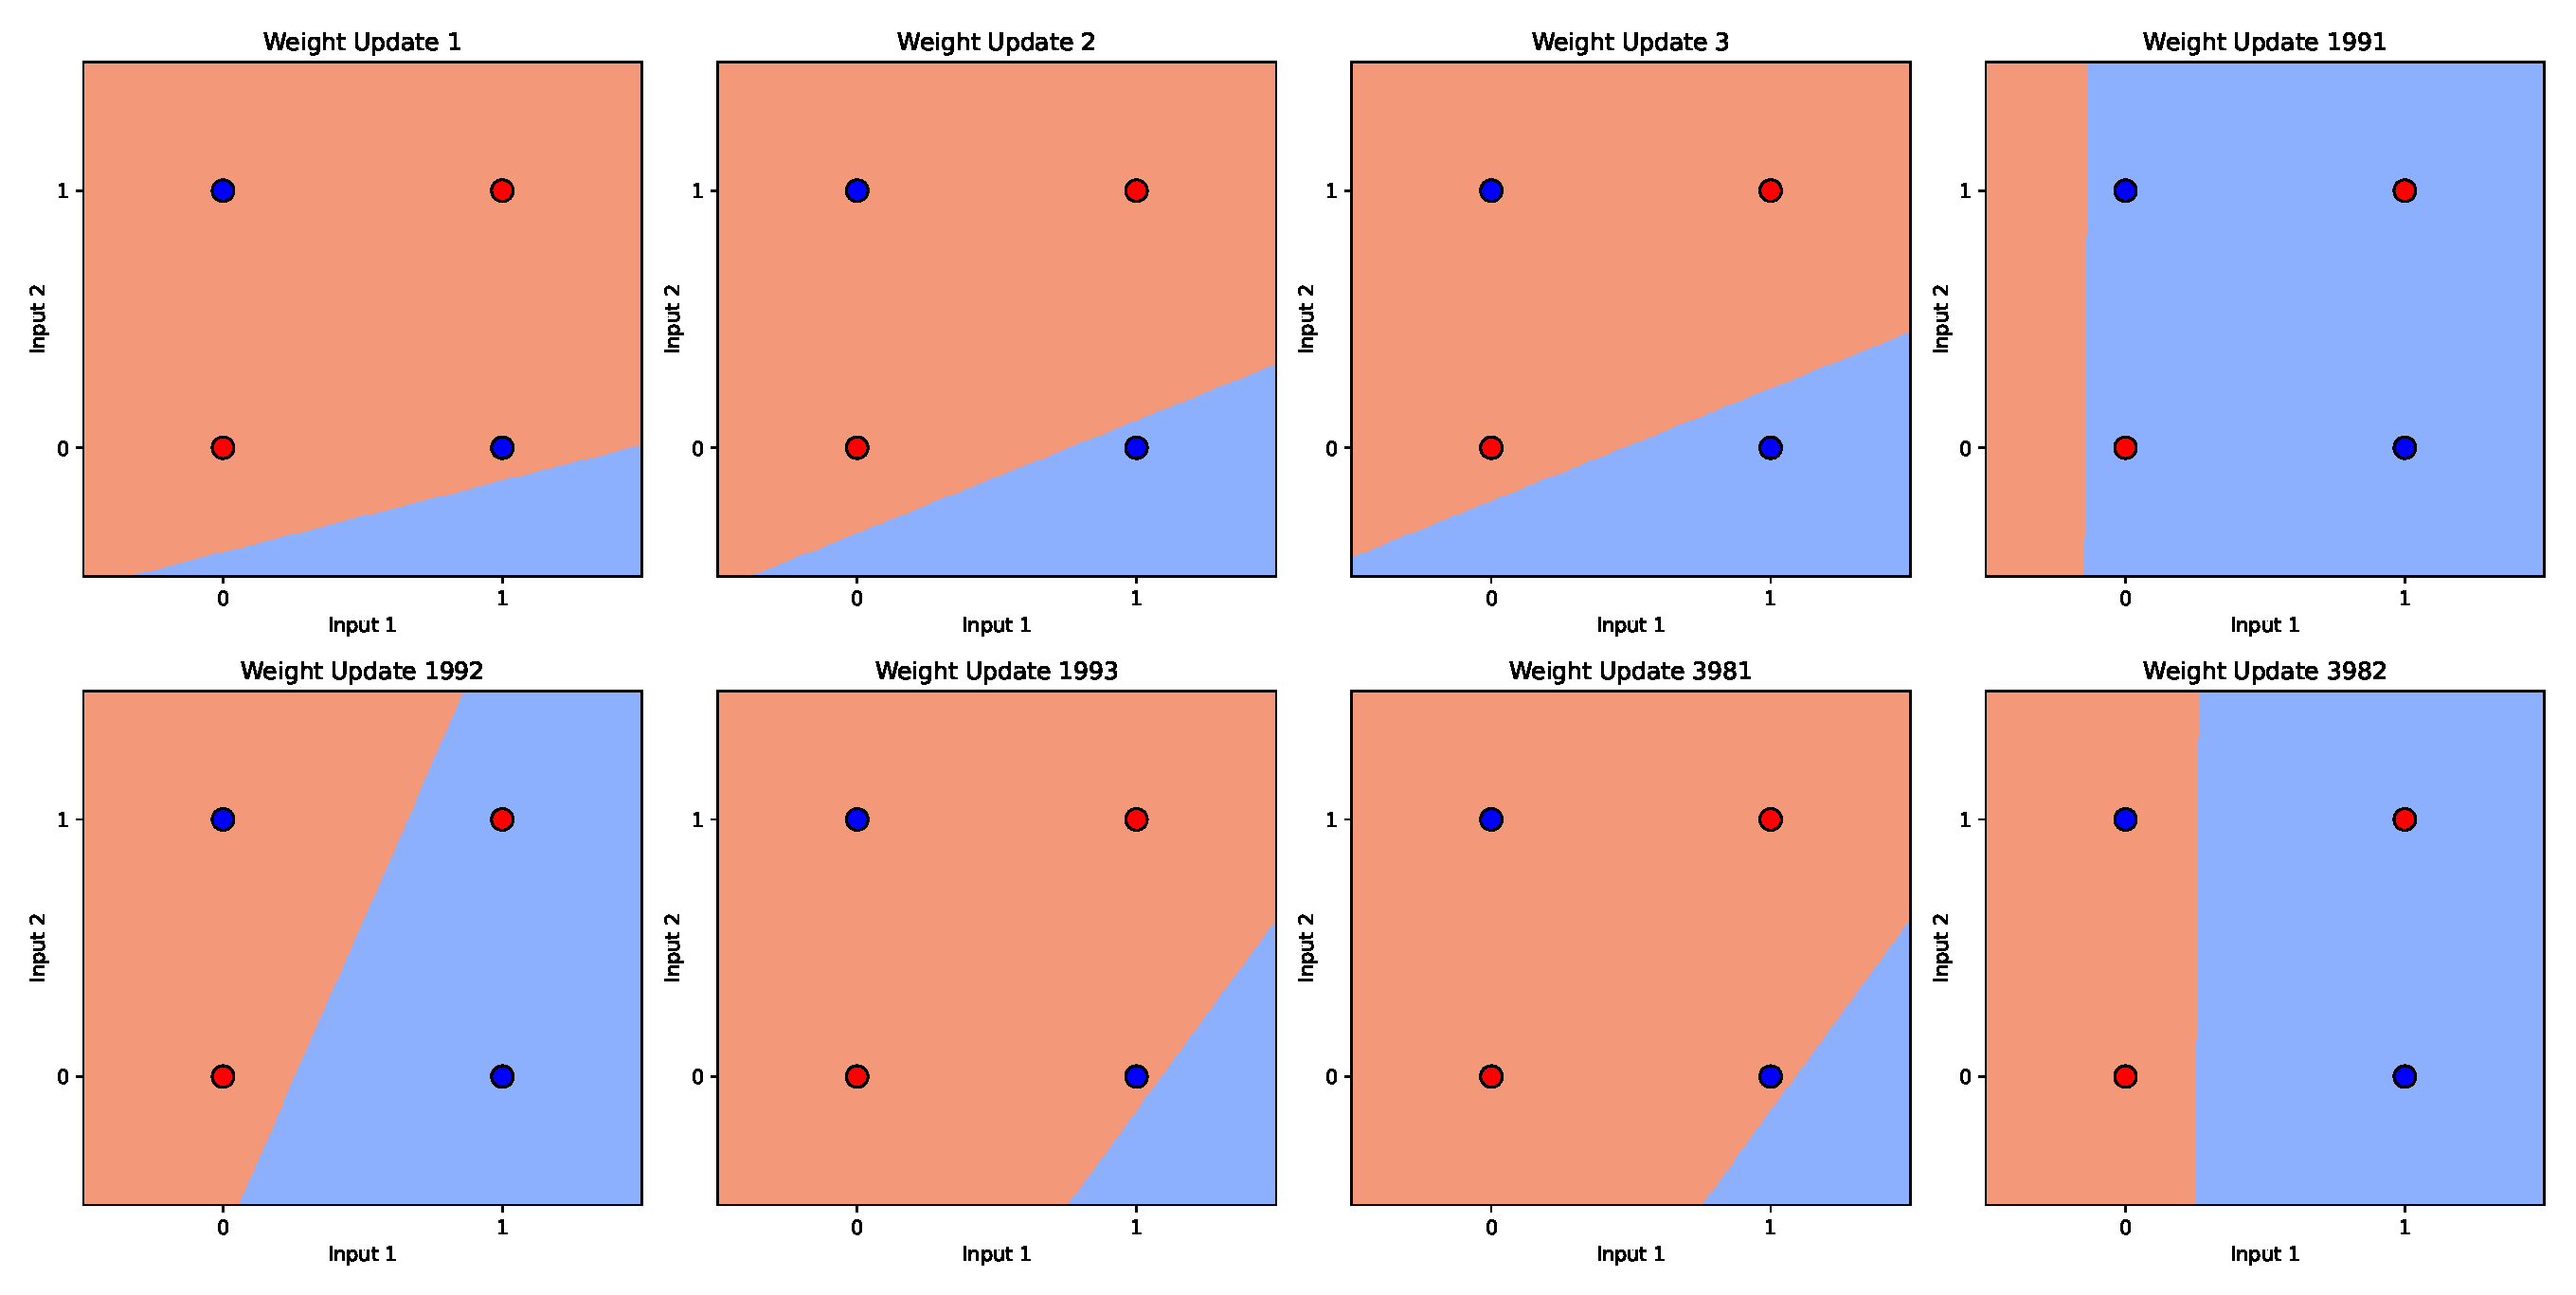
\includegraphics[width=\textwidth]{XOR_Decision_Boundaries.eps}
\caption{Decision Boundaries for XOR Gate}
\end{figure}

\textbf{Interpretation:}

As the training goes on, the perceptron keeps updating its weights and hence the decision boundary changes. However, the boundary neither stabilises nor correctly classifies all four xor input combinations. This shows that the algorithm does not converge.

\textbf{Analysis:}

The XOR problem is not linearly separable, so you can not separate its classes with a single straight-line decision boundary. The perceptron updates the weights to correct one misclassified sample but in turn misclassifies another sample. This leads to continuous oscillation of the weights and no convergence.

\section*{11. Conclusion}

A Multi-Layer Perceptron (MLP) model has been successfully built for multi-class classification of images based on the Fashion-MNIST data set. The images in the data set were preprocessed in terms of flattening, normalization, and one-hot encoding of the labels. The baseline model obtained good classification results and RandomizedSearchCV with the help of the SciKeras package was applied for automatic tuning of hyperparameters. The tuned model obtained 88.63\% cross-validation accuracy which is comparable to the baseline model's test accuracy.

\section*{12. References}
\begin{enumerate}
\item Goodfellow et al., \emph{Deep Learning}.
\item Bishop, \emph{Pattern Recognition and Machine Learning}.
\item Haykin, \emph{Neural Networks and Learning Machines}.
\item Fashion-MNIST Dataset.
\item TensorFlow/Keras Documentation.
\end{enumerate}

\end{document}
